% !TEX program = lualatex

\documentclass[
11pt,
captions=tableheading,
%smallheadings,
%headings=big,
headsepline,
footsepline, 
%chapterprefix=false			% weiss nicht was passiert
captions=tableheading,
parskip=half-,
%BCOR=10mm,
%twocolumn, 
%draft
]{scrartcl}

%\usepackage[babelshorthands]{polyglossia}
\usepackage{polyglossia}
\setdefaultlanguage[variant = swiss]{german}

%\usepackage[ngerman]{babel} 
\usepackage[]{ scrlayer-scrpage }
\usepackage[ a4paper,
total={165mm,244mm},
 left=25mm,
 top=25mm,
 headsep=10mm
 %footsep=12mm
 %,showframe
  ]{geometry}
 \usepackage{fontspec}
\setmainfont{Times New Roman}
\setsansfont{Arial}

\usepackage[dvipsnames]{xcolor}
\usepackage[most]{tcolorbox}
\usepackage[
version=3,
arrows=pgf-filled,
]{mhchem} % für chemische Formeln
\usepackage{microtype}
\usepackage{float}
\usepackage{enumitem}
\usepackage{multicol}
\usepackage{booktabs}
\usepackage{pgfplots}
\usepackage{tabularx}
\usepackage{longtable}
\usepackage{fontawesome5}
\usepackage{pdfpages}

\usepackage{pdflscape} % Für Querformat-Seiten


\usepackage{siunitx}
\usepackage{amsfonts}
\usepackage{tabularx}

%Quellen 
\usepackage[
    backend=bibtex, 
    natbib=true,
    style=numeric,
    sorting=none
]{biblatex}
\addbibresource{../Quellen.bib}

\usepackage[section]{placeins} % avoids images in the wrong section



% order of hyperref, cleverref is important
\usepackage[hidelinks]{hyperref}
\usepackage{cleveref}



\frenchspacing



\floatplacement{figure}{H}

% Labeling of elements
\counterwithin{figure}{section}
\counterwithin{table}{section}
\counterwithin{equation}{section}

% Colors
\definecolor{blau_bauschule}{RGB}{22,65,148}

% Titel mit Bauschule blau gemäss CI manual
\addtokomafont{section}{\color{blau_bauschule}\Huge}
\addtokomafont{subsection}{\color{blau_bauschule}\huge}
\addtokomafont{subsubsection}{\color{blau_bauschule}\Large}
\addtokomafont{paragraph}{\normalsize}
\addtokomafont{subparagraph}{\small}
% Pagestyle
\pagestyle{scrheadings}
\ihead{\fontsize{9pt}{2pt}\selectfont }
\ohead{\fontsize{9pt}{2pt}\selectfont Baustoffe}
\chead{\fontsize{9pt}{2pt}\selectfont \headmark}
\ifoot{\fontsize{9pt}{2pt}\selectfont Bauschule Aarau} 
\ofoot{\fontsize{9pt}{2pt}\selectfont \thepage} %Seitennummer
\cfoot{\fontsize{9pt}{2pt}\selectfont }
\setkomafont{pagehead}{\normalfont}
\setkomafont{pagefoot}{\normalfont}
\setkomafont{pagefoot}{\normalfont}
\setkomafont{pagehead}{\normalfont}
\setkomafont{pagefoot}{\normalfont}
\setcounter{topnumber}{1}
\setcounter{bottomnumber}{1}
\automark[section]{subsection}


% Bild- und Tabellenunterschriften
\renewcommand*{\figurename}{Abbildung}
\renewcommand*{\tablename}{Tabelle}


% Titel
\title{Baustoffe}
%\author{Patrick Pfändler}
\date{2021}

% https://tex.stackexchange.com/questions/501018/how-to-write-a-minitoc-with-plain-koma-script

%https://www.mrunix.de/forums/archive/index.php/t-74962.html


\makeatletter
\newcommand\reaction@[1]{\begin{equation}\ce{#1}\end{equation}}
\newcommand\reaction@nonumber[1]%
{\begin{equation*}\ce{#1}\end{equation*}}
\newcommand\reaction{\@ifstar{\reaction@nonumber}{ \reaction@}}
\makeatother
%renewtagform{reaction}[R ]{(}{)}

%% Custom icons 
\newcommand{\Lerniziel}{\faBullseye}
\newcommand{\Diskussion}{\faComments}
\newcommand{\TR}{\faCalculator}
\newcommand{\Fragen}{\faQuestionCircle}
\newcommand{\LeherTafel}{\faChalkboardTeacher}








\begin{document}


\pagestyle{scrheadings}

% Commands
\newcommand{\myNmm}[1]
{
\sisetup{per-mode=symbol}
\SI{#1}{\newton\per\mm\squared}
}


\newcommand{\kommzerielleProdukte}[1]
{
    \textcolor{Brown}{Kommerzielle Produkte:}  #1
}




%\renewcommand{\familydefault}{\sfdefault}
%\setkomafont{captionlabel}{\itshape \fontsize{10pt}{2pt}}
%\setkomafont{caption}{\sffamily} 

\newtcolorbox{Definition}[1]{
colback=green!5!white,
colframe=green!75!black,fonttitle=\bfseries,
title=#1}


\newtcolorbox{Merke}{
enhanced,
boxrule=0pt,frame hidden,
borderline west={4pt}{0pt}{red!75!black},
colback=white,
sharp corners
}

\newtcolorbox{Masseinheit}[1]{
enhanced,
boxrule=1pt,colframe=blue,
colback=white,
sharp corners, 
colframe=blue!75!black,
title = #1, 
after title={\hfill\colorbox{ NavyBlue}{Masseinheit}}
}

\newtcbox{\ExampleSimple}[1][gray]{on line,
arc=0pt,outer arc=0pt,colback=#1!10!white,%colframe=#1!50!black,
frame hidden,
boxsep=0pt,left=1pt,right=1pt,top=1pt,bottom=1pt,
boxrule=0pt,bottomrule=1pt,toprule=1pt}

%\maketitle
{\color{blau_bauschule}\fontsize{30pt}{21pt}\selectfont \textbf{Dokumentierter Unterrichtsbesuch}}





\section*{Übersicht}

\begin{table}[ht]
    \centering
    \label{tab:uebersicht}
    \begin{tabularx}{\textwidth}{@{}Xp{11cm}@{}}
    \toprule
    Lehrperson: & Patrick Pfändler \\
    Studiengang: & HFP Bauführung \\
    Fach: & Baustoffe \\
    \midrule
    Klasse: & HTf-26 \\
    Semester: & 1 \\
    Anzahl Schüler: & 14 \\
    Ort: & Bauschule Aarau \\
    Datum: & 16.12.2024 \\
    Uhrzeit: & 08:00 - 10:00 \\
    Unterrichtszeit: & 2 Stunden \\
    Schulzimmer: & 301 \\
    Schulzimmerausrüstung: & Beamer (2x), Hellraumprojekterersatz, Flipchart \\
    \midrule
    Persönliche Ausrüstung: & Laptop, Pointer, IPad \\
    \midrule
    Inhalt der Lektion: & Carolabrücke, Korrosionsbeständige Bewehrung, Betoninstandsetzung \\
    \bottomrule
    \end{tabularx}
    \end{table}

    \begin{tcolorbox}[colback=blue!5!white, colframe=blue!75!black, title=CHANGELOG]
        \textbf{14.12.2024:} Update Dokument mit Updates zur Carolabrücke.

        \textbf{17.12.2024:} Update Dokument mit Reflexion
        \end{tcolorbox}


\clearpage
\vspace*{2cm}
\setcounter{tocdepth}{3} % Tiefe des Inhaltverzeichnisses steuern
\tableofcontents%
\clearpage

\subsection*{Abkürzungsverzeichnis}
\begin{table}[H]
    \centering
    \label{tab:abkuerzungen}
    \begin{tabularx}{\textwidth}{@{}ll@{}}
    \toprule
    %\midrule
    Bsp. & Beispiel \\
    BS & Baustoffe \\
    LP & Lehrperson \\
    SF & Sozialform \\
    FK & Fachkompetenz \\
    OS & Oberflächenschutzsystem \\
    GFK & Glasfaserverstärkter Kunststoff \\
    ASTRA & Bundesamt für Strassen \\
    \bottomrule
    \end{tabularx}
    \end{table}



\clearpage

\section{Bedigungsanalyse}

\subsection{Zielgruppenanalyse}
Die Zielgruppen sind angehende Bauführer und Bauführerinnen. Die Studierenden sind zwischen 20 und 30 Jahre alt und haben meistens eine abgeschlossene Berufslehre als Maurer, teilweise eine abgeschlossene Weiterbildung zum Polier oder Vorarbeiter (inkl. Berufsbildnerkurs). 
Teilweise gibt es ältere Studierende, welche aufgrund eines gesundheitlichen Leidens von der IV an die Bauschule Aarau überwiesen wurden um dort die Ausbildung zum Bauführer zu absolvieren.
Aus diesen Gründen kann die Motivation sowohl intrinsisch als auch extrinsisch sein.
Sie verfügen über praktische Erfahrung im Baugewerbe und haben bereits erste Erfahrungen in der Bauführung in den Unternehmen gesammelt.

Schlussendlich soll der Unterricht eine Vorbereitung auf die eidgenössische Prüfung zum Bauführer sein. 
Vor der eigenössischen Prüfungen findet nochmals ein Repetitionsblock statt. 

Die Vorkenntnisse können aufgrund vorhandener oder nicht vorhandener Weiterbildungen sehr unterschiedlich sein. 
Ebenfalls besteht eine grosse Heterogenität in den Lernvoraussetzungen, da die Studierenden aus unterschiedlichen Berufsfeldern (Quereinsteiger) kommen können.

Die Arbeit auf Baustellen setzt voraus, dass sich die Studierenden Teamfähigkeiten aneignen und sich in einem Team integrieren können. 

Die Studierenden sind sich besonders anfangs nicht mehr gewöhnt den ganzen Tag zu sitzen und im Schulzimmer zu verbringen. 
Die Kenntnisse in der Anwendung von digitalen, kollaborativen Tools sind unterschiedlich ausgeprägt.
Die Selbstorganisation der Studierenden ist unterschiedlich ausgeprägt, je nach Ausbildungsstand. 
Die Meisten müssen sich in der Selbstorganisation erst wieder zurechtfinden.

\subsection{Rahmenbedingungen}
\subsubsection{Strukturelle Rahmenbedingungen}
Das Zeitbudget für die Unterrichtszeit beträgt 2 Stunden. Der Unterricht findet in der Bauschule Aarau statt. Die Schülerzahl beträgt 14 Personen. Der Unterricht beginnt um 08:00 Uhr und endet um 10:00 Uhr.
Die Lektion startet überlicherweise im Schulzimmer.

Die Studierenden haben eine fixes Schulzimmer zugeteilt und eine fixe Sitzordnung. Der Lehrerpult befindet sich vorne in der Mitte des Raumes. Der Beamer ist an der Decke montiert und kann über ein Kabel mit dem Laptop verbunden werden. Ein Hellraumprojektor ist ebenfalls vorhanden. Ein Flipchart steht zur Verfügung.


Die Studierenden arbeiten in der Regel mit einem Laptop und einem Tablet. Einzelne Studiererende drucken die Unterlagen aus. 
Für einige Aufgaben wird ein Taschenrechner vorausgesetzt.

\subsection{Jahresplanung}
Für das Fach Baustoffe stehen rund \SI{64}{\hour} Unterrichtszeit zur Verfügung.
Diese Lektion ist die letzte Doppelstunde im Fach Baustoffe. 
Weitere Lektionen bei dieser Klasse sind erst im Jahr 2025 geplant. 
Die genannten Lektionen sollen dann spezifisch auf die HFP Prüfung vorbereiten. Aktuell gibt es leider keine Musterprüfungen für die HFP Prüfung. Diese wurden 2024 erwartet, sind aber noch nicht verfügbar.

Die Anzahl der Lektionen hat sich im Verlauf des Semesters auf über \SI{80}{\hour} erhöht und die Planung musste angepasst werden.

\subsection{Berufspädaogisches Konzept}
\subsubsection{Kognitive Taxonomiestufen nach Bloom}

\begin{table}[H]
    \centering
    \label{tab:Bloom}
    \caption{Kognitive Taxonomiestufen nach Bloom \cite{bloom1956taxonomy}, adaptiert von \cite{BerufspädagogischesKonzept_BauschuleAarau}.}
    \begin{longtable}{@{}llp{12cm}@{}}
        \toprule
        \textbf{Stufen} & \textbf{Begriff} & \textbf{Beschreibung} \\ 
        \midrule
        K1 & Wissen & Sie geben gelerntes Wissen wieder und rufen es in gleichartiger Situation ab. \\ 
        K2 & Verstehen & Sie erklären oder beschreiben gelerntes Wissen in eigenen Worten. \\ 
        K3 & Anwenden & Sie wenden gelernte Technologien/Fertigkeiten in unterschiedlichen Situationen an. \\ 
        K4 & Analyse & Sie analysieren eine komplexe Situation, d.h. sie gliedern Sachverhalte in Einzelelemente, decken Beziehungen zwischen Elementen auf und finden Strukturmerkmale heraus. \\ 
        K5 & Synthese & Sie kombinieren einzelne Elemente eines Sachverhalts und fügen sie zu einem Ganzen zusammen. \\ 
        K6 & Beurteilen & Sie beurteilen einen mehr oder weniger komplexen Sachverhalt aufgrund von bestimmten Kriterien. \\ 
        \bottomrule
    \end{longtable}
\end{table}




\subsubsection{RITA-Modell}
Die Lektion wird nach dem RITA-Modell durchgeführt. 
Die Studierenden werden mit konkreten Aufgaben aus der Praxis konfrontiert und ihr Vorwissen, Erfahrungen, Haltungen zum Thema oder gar erste Problemlösungen werden aktiviert.
Diese Rythmisierte Unterrichtsablauf wird in der Tabelle \cref{tab:RITA_Modell} dargestellt und ist Teil des berufspädagogischen Konzepts der Bauschule Aarau \cite{BerufspädagogischesKonzept_BauschuleAarau}


\begin{table}[H]
    \centering
    \label{tab:RITA_Modell}
    \caption{RITA-Modell, adaptiert von \cite{BerufspädagogischesKonzept_BauschuleAarau}.}
    \begin{tabularx}{\textwidth}{@{}llp{9.5cm}@{}}
    \toprule
    \textbf{Phase} & \textbf{Beschreibung} & \textbf{Umschreibung} \\
    \midrule
    R:  & Ressourcen aktivieren & Studierende werden mit konkreten Aufgaben aus der Praxis konfrontiert; Vorwissen, Erfahrungen, Haltungen zum Thema oder gar erste Problemlösungen werden aktiviert. \\
    I: & Informationen verarbeiten & {} \\
    T: & Transfer anbahnen & {} \\
    A: & Auswerten & {} \\
    \bottomrule
    \end{tabularx}
    \end{table}


\clearpage


\section{Lektionsplanung}
\subsection{Fachliche Grundlagen}
Die Studierenden hatten über \SI{60}{\hour} das Fach Baustoffe. 
Sämtliche Themen wurden bereits abgehandelt, sowohl formativ als auch summativ geprüft. 

Die nächste Prüfung wird den Studierenden jeweils bekannt gegeben. 
Verschiebung der Prüfungstermine sind nach Rücksprache mit der LP möglich.



\subsection{Lernziele}
\subsubsection{Fachkompetenzen}
Die Studierenden repetieren die wichtigsten Themen des Fachs Baustoffe.
Die Lernziele \faBullseye\, für die einzelnen Themen sind den Studierenden bekannt.



\subsection{Sozialform}
Die Sozialform ist in den meisten Fällen Frontalunterricht. 
Die Studierenden sitzen im Schulzimmer und hören der Lehrperson zu. Es wird auf eine aktive Beteiligung der Studierenden geachtet und aktive gefördert. 

Gemäss meinen eigenen Zielen für den Didaktikkurs sollen zusätzliche Medien im Unterricht verwendet werden, als auch Gruppenarbeiten durchgeführt werden.

\subsection{Medieneinsatz}
Der Beamer wird häufig für die Präsentation der Lerninhalte verwendet. 
Ein Hellraumprojektor steht als Ersatz zur Verfügung. Ein Flipchart wird für die Visualisierung von Inhalten bei Bedarf verwendet.

\subsection{Grobplanung der Unterrichtseinheit}
\subsubsection{Stand von letzter Woche}
In der letzten Woche konnte der Unterricht nicht abgeschlossen werden.
Die Studierden hatten sich sehr aktiv beteiligt, Inputs eingebracht und Fragen gestellt. 
Aus diesen Gründen musste das Video zu korrosionsbeständiger Bewehrung nach rund \SI{15}{\min} auf die nächste Lektion verschoben werden.
Eine kurze Sachanalyse wurde durchgeführt und befindet sich im Anhang \cref{sec:Sachanalyse}.

\subsubsection{Inhalte der Lektion}
\begin{itemize}
    \item Aktivierung der Studierenden mit Repetitionsfragen und Rechenaufgaben zur letzten Lektion mit Folien (\textit{Ressourcen aktivieren})
    \item Weitergehen mit dem Video (Minute 16 bis 48) zu korrosionsbeständiger Bewehrung (\textit{Information verarbeiten})
    \item Diskussion über die Vor- und Nachteile von korrosionsbeständiger Bewehrung (\textit{Transfer anbahnen})
    \item Praktische Umsetzung des gelernten anhand von Beispielen aus der Praxis als Gruppenarbeit (\textit{Auswerten})
\end{itemize}

\subsubsection{Ziele der Lektion}
Für die Lektion sind folgende Ziele definiert:
\begin{itemize}
    \item Kenntnisse über die Möglichkeiten korrosionsbeständiger Bewehrungsmaterialien
          \begin{itemize}
              \item Nicht-rostender Betonstahl
              \item Faserbewehrung
                    \begin{itemize}
                        \item Glasfaser-Bewehrung
                        \item Carbonfaser-Bewehrung
                        \item Basalfaser-Bewehrung
                    \end{itemize}
          \end{itemize}
\end{itemize}


\subsubsection{Mikroebene}
Diese Lektion ist die letzte Lektion im Fach Baustoffe vor den Weihnachtsferien. 
Die Studierenden sind üblicherweise nicht mehr so fokussiert und häufig stehen noch Prüfungen in anderen Fächern an. 

\subsubsection{Spezielles}
Ein Studierender kann derzeit nicht physisch am Unterricht teilnehmen und wird daher über Teams zugeschaltet. 
Die Lehrperson hat die Möglichkeit, den Studierenden über Teams zuzuschalten. 
Der Unterricht wird aber nicht ausgelegt auf einen Hybridunterricht.


\textbf{Nachtrag: Carolabrücke}
Erster Bericht zur Carolabrücke wurde freigegeben. 
Das Thema des Einsturzes ware vor den Herbstferien ein Thema im Unterricht und soll daher nochmals aufgegriffen werden.




\begin{landscape}
\subsection{Verlaufsplanung}
\begin{longtable}{@{}l|p{9cm}p{7.5cm}p{3.5cm}@{}}
    \toprule
    \textbf{Zeit} & \textbf{Aktivität der Lehrperson} & \textbf{Aktivitäten der Studierenden} & \textbf{Medieneinsatz} \\
    \midrule
    \endfirsthead
    \toprule
    \textbf{Zeit} & \textbf{Aktivität der Lehrperson} & \textbf{Aktivitäten der Studierenden} & \textbf{Medieneinsatz} \\
    \midrule
    \endhead
    \midrule
    \multicolumn{4}{r}{\textit{Fortsetzung auf der nächsten Seite}} \\
    \midrule
    \endfoot
    \bottomrule
    \endlastfoot
    \midrule
    08:00 - 08:05 & \textbf{Einstieg: }Begrüssung der Studierenden und Vorstellung von Natalie Raeber; Anschliessend vorstellen des Programms; Abholen, ob Fragen zur Lektionsinhalt bestehen; Webuntis: Erfassen der Absenzen; Skizzieren des Stundenablaufs mit PP & Begrüssung der Lehrperson und vorbereiten der Unterlagen; Hören der LP zu. & Beamer mit PP-Folien und Zuschalten von Alessandro auf Teams\\
    \midrule
    08:05 - 08:15 & \textbf{Aktivierung: } Input zur Carolabrücke (Resultate der Analyse) & Aktives Zuhören und Notizen machen (nach Bedarf) & Beamer mit PP-Folien und 2min 30 s Video\\
    \midrule
    08:15 - 08:35 & \textbf{Aktivierung:} Repetitionsfragen zur letzten Lektion und Rechenaufgaben zur korrosionsbeständigen Bewehrung; (Details auf den Folien) & Beantworten der Fragen und lösen der Rechenaufgaben  & Beamer mit PP-Folien\\
    \midrule
    08:35 - 09:10 & \textbf{Information:} Video zu korrosionsbeständiger Bewehrung (Minute 16 bis 48) & Schauen des Videos und Notizen machen & Beamer mit Video\\
    \midrule
    09:10 - 09:20 & \textbf{Pause:} evtl. bereits Video unterbrechen {} & {}\\
    \midrule
    09:20 - 09:25 & \textbf{Transfer:} Diskussion über die Vor- und Nachteile von korrosionsbeständiger Bewehrung; Eindrücke zum Video; ggf. Verknüpfung mit bereits durchgeführten Lektionen im Fach BS & Diskussion in der Klasse & {}\\
    \midrule
    09:25 - 09:30 & \textbf{Transfer:} Diskussion über das Lösen von Dauerhaftigkeitigkeitsproblemen in der Praxis; Wie sichert ihr die Dauerhaftigkeit auf der Baustelle. Prüfen, wie in den Gruppen gearbeitet wird. & Diskussion in der Klasse & Nach Bedarf Ipad oder Flipchart oder Folien \\
    \midrule
    09:30 - 09:45 & \textbf{Transfer:} Gruppenarbeit (2-er): Wo könnt ihr in eurem Arbeitsalltag vorstellen eine alternavtive Form der Bewehrung zu verwenden? & Bearbeiten der Aufgaben in Gruppen & Nach Bedarf Ipad oder Flipchart oder Folien\\
    \midrule
    09:45 - 09:50 & \textbf{Transfer:} Diskussion der Gruppenarbeiten im Plenum  & Aktives zuhören; Vorstellen der eigenen Gruppenarbeit & Nach Bedarf Ipad oder Flipchart oder Folien\\
    \midrule
    09:50 - 09:55 & \textbf{Abschluss:} Zusammenfassung der wichtigsten Punkte von heute; Ausblick auf die nächsten Wochen nach den Ferien; evtl. Quiz nach den Ferien zum Thema (als foramtive Leistungsüberprüfung)& Zuhören & Beamer mit PP resp. PDF mit Semesteprogramm\\
    \midrule
    09:55 - 10:00 & \textbf{Abschluss:} Verabschiedung der Studierenden & Zusammenpacken der Unterlagen im Fach BS und Verabschiedung der LP & Beamer mit PP-Folien\\
    \midrule
    %\Xhline{2\arrayrulewidth} % A thick line that is twice the default thickness
    \\ \addlinespace
    \midrule
    10:00 - 10:15 & \textbf{Backup Material:} Weiter mit dem Folien zu den Instandsetzungskonzepten. & nächste Unterrichtsstunde startet & {}\\
    \midrule
    10:00 - 11:00 & \textbf{Nachbereitung:} Feedbackrunde mit Natalie Raeber & nächste Unterrichtsstunde startet & {}\\
    \midrule
    später & \textbf{Nachbereitung:} Optimieren der Lektion & nächste Unterrichtsstunde startet & {}\\
    \bottomrule
\end{longtable}
\end{landscape}
\clearpage

\begin{landscape}
    
    \section{Reflexion}
    \subsection{Selbstreflexion}
    \Cref{tab:Reflexion} zeigt die Selbstreflexion zur Unterrichtsplanung und -durchführung.
    
    \begin{longtable}{@{}p{8cm}|p{15cm}@{}}
        \caption{Selbstreflexion zur Unterrichtsplanung und -durchführung} \label{tab:Reflexion} \\ % Proper caption placement
        \toprule
        \textbf{Reflexionsbereich} & \textbf{Inhalte und Beobachtungen} \\
        \midrule
        \endfirsthead % Start of the first page header
        \multicolumn{2}{c}{\textit{Fortsetzung der Tabelle \ref{tab:Reflexion}}} \\
        \toprule
        \textbf{Reflexionsbereich} & \textbf{Inhalte und Beobachtungen} \\
        \midrule
        \endhead % Start of subsequent pages header
        \midrule
        \multicolumn{2}{r}{\textit{Fortsetzung auf der nächsten Seite}} \\
        \midrule
        \endfoot
        \bottomrule
        \endlastfoot
    
        % --- Table Content ---
        Didaktische Entscheidungen reflektieren, Zielerreichung analysieren, Optimierungsbedarf benennen und begründen &
        \begin{itemize}
            \item Quiz erstellen für einen formativen Test, um den Lernfortschritt individuell zu überprüfen.
            \item Video ggf. häufiger unterbrechen und Position der Lehrperson anpassen, um die Studierenden besser zu beobachten.
            \item Lernziele didaktisch feiner aufbereiten (Hinweis: vgl. Liste mit Verben für die unterschiedlichen Taxonomiestufen). Entscheidung zwischen "Tiefe" oder "Breite" während meiner Vorbereitung treffen.
            \item Eigene Fragen nicht zu schnell selbst beantworten.
            \item Die hinterste Reihe aktiv einbeziehen und sicherstellen, dass niemand ignoriert wird oder sich ignoriert fühlt.
        \end{itemize} \\
        \midrule
    
        Planung und Durchführung vergleichen und Abweichungen differenziert begründen &
        \begin{itemize}
            \item Gruppenarbeit (2-er Teams) konsequent einfordern, auch wenn es die Unterrichtseinheit verlängert. Studirende brauchen etwas Zeit um den Input zu verarbeiten
            \item Aktives Zuhören aktiver einfordern: Notizen erstellen und ggf. schriftliche Aufträge formulieren.
            \item  Wichtigste Punkte für nach den Ferien zwingend mündlich festhalten oder zumindest auf die Folien hinweisen.
        \end{itemize} \\
        \midrule
    
        Eigenes Handeln als Lehrperson im Hinblick auf das Lernen der Schülerinnen und Schüler reflektieren, Handlungsalternativen entwickeln und begründen &
        \begin{itemize}
            \item Eigene Position im Raum mehr variieren.
            \item Siehe vorherige Punkte für Anpassungen.
        \end{itemize} \\
        \midrule
    
        Entwicklungsziele und nächste Schritte formulieren und begründen &
        \begin{itemize}
            \item Stärker bei Nichtbeteiligung der Studierenden durchgreifen.
            \item Lernziele nochmals überarbeiten und konkretisieren.
            \item Summatives Quiz erstellen.
            \item Video stärker zur Beobachtung der Studierenden nutzen und ggf. häufiger unterbrechen.
            \item Übung einfügen: Beispiel eines Baustellenfotos mit erkennbaren Fehlern, um K3-Niveau (Anwenden) zu erreichen.
            \item Wichtigste Punkte für nach den Ferien zwingend mündlich festhalten oder zumindest auf die Folien hinweisen.
        \end{itemize} \\
    \end{longtable}
    \end{landscape}
    





\clearpage
\addcontentsline{toc}{section}{Literatur}

\printbibliography
\clearpage
\section*{Anhang}
\addcontentsline{toc}{section}{Anhang}

%\subsection*{Grobplanung}
%\addcontentsline{toc}{subsection}{Grobplanung}

%\clearpage
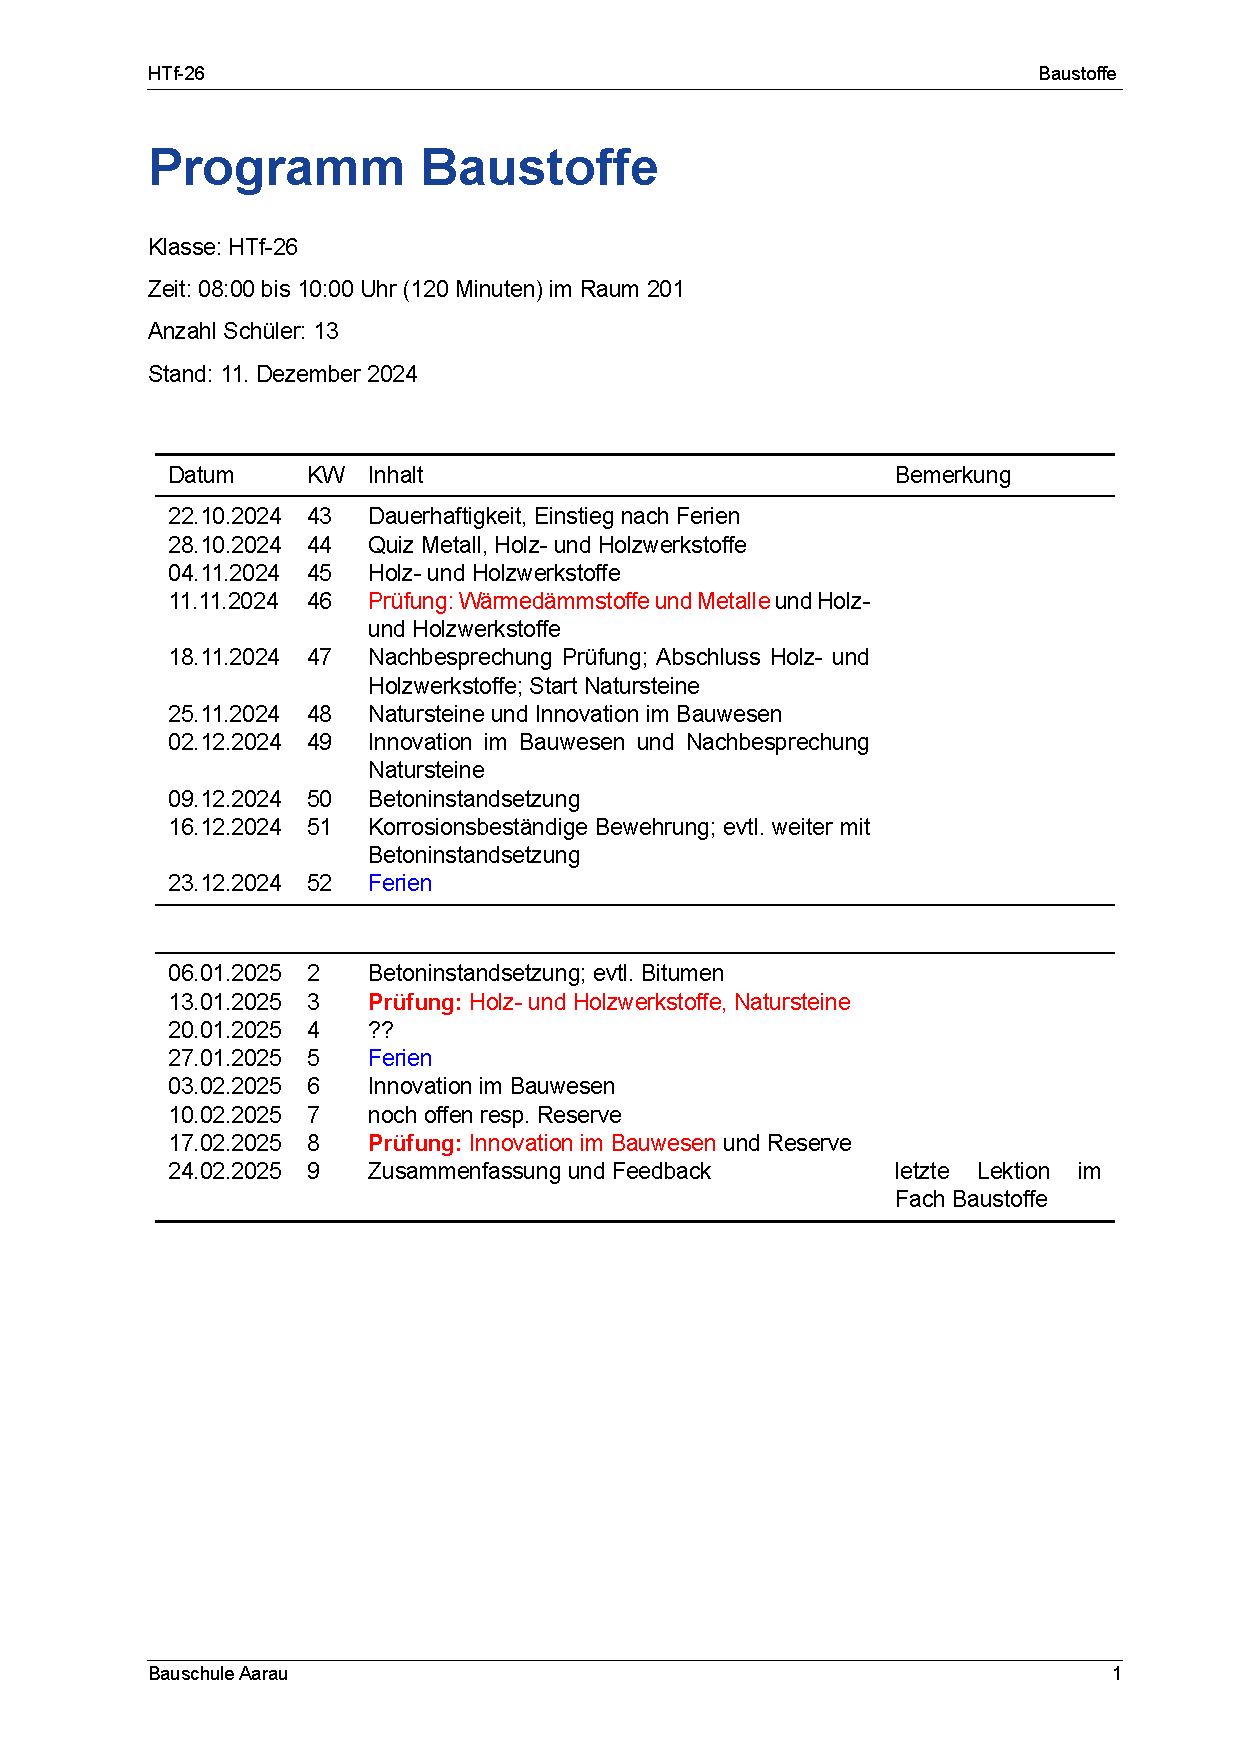
\includepdf[pages=-]{../../HTf-26/Programm/Programm_HTf-26.pdf}

%\section*{Lernziele}
%\addcontentsline{toc}{subsection}{Lernziele}

%Beispiel von Lernzielen einer Prüfung:
%\clearpage
%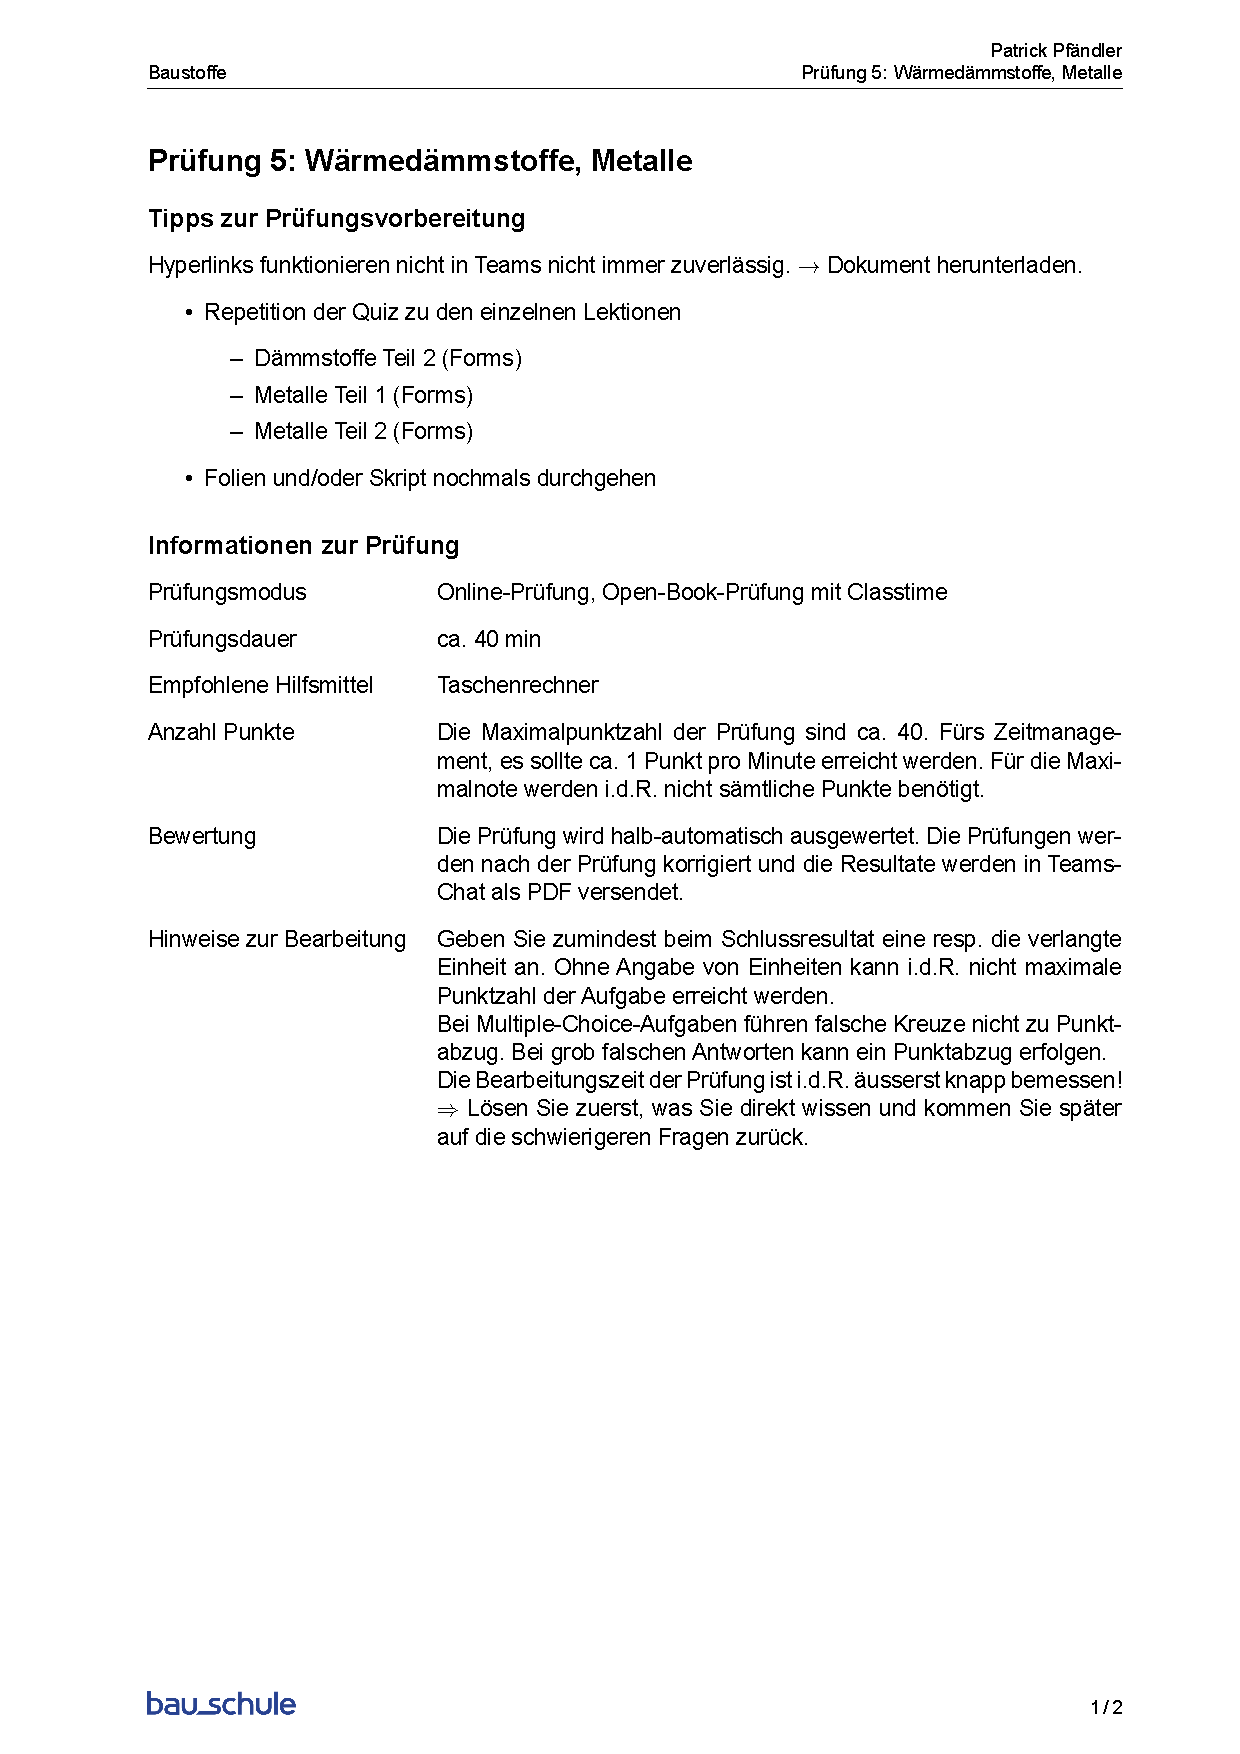
\includepdf[pages=-]{../..//HTf-26/WDS_Metall/Pr5_WDS_Metalle_Lernziele.pdf}
\subsection*{Sachanalyse}
\label{sec:Sachanalyse}
\addcontentsline{toc}{subsection}{Grobplanung}
Im folgenden wird die Sachanalyse kurz skiziert.


\begin{itemize}
    \item \textbf{Grundlagen:} Korrosionsbeständige Bewehrung ist eine Bewehrung aus Stahl oder anderen Materialien, die so beschaffen ist, dass sie besonders widerstandsfähig gegen Korrosion (Rostbildung) ist. Diese Art von Bewehrung wird insbesondere in Bereichen eingesetzt, in denen aggressive Umwelteinflüsse wie Chloride (z.\,B. Streusalz) oder Kohlendioxid das Risiko für Korrosion erhöhen.
    
    \item \textbf{Hintergrund:} In Stahlbetonbauwerken dient Beton als alkalisches Schutzmedium für den Stahl. Der hohe pH-Wert im Beton sorgt dafür, dass der Stahl durch eine natürliche Passivschicht geschützt bleibt. Sobald der pH-Wert aufgrund von Karbonatisierung oder durch das Eindringen von Chloriden sinkt, wird die Passivschicht zerstört und Korrosion kann einsetzen. Dies führt zu einer Reduzierung der Tragfähigkeit und erhöhten Instandhaltungskosten.

    \item \textbf{Materialien:}
    \begin{itemize}
        \item \textit{Niedrig- oder hochlegierter Stahl (nichtrostender Stahl):} Enthält höhere Anteile an Chrom , Nickel und oft Molybdän. Diese Legierungskomponenten bilden eine stabile Passivschicht auf der Oberfläche, die den Stahl vor Korrosion schützt. Diese Bewehrung wird oft in Brücken oder maritimen Bauwerken eingesetzt.
        \item \textit{Verzinkter Stahl:} Der Stahl wird mit einer Zinkschicht versehen, die als Opferanode dient. Die Zinkschicht korrodiert zuerst und schützt so den darunterliegenden Stahl. Diese Methode ist kostengünstiger als nichtrostender Stahl, hat jedoch eine begrenzte Lebensdauer.
        \item \textit{Epoxidharz-beschichteter Stahl (Epoxy Coated Rebars):} Der Stahl wird mit einer Epoxidschicht überzogen, die das Eindringen von Wasser und Chloriden verhindert. Diese Methode ist besonders geeignet für Bereiche mit hoher Chloridbelastung, z.\,B. Parkhäuser oder Strassenbauwerke.
        \item \textit{Faserverbundwerkstoffe (z.\,B. GFK-Bewehrungen):} Diese bestehen aus Glas- oder Carbonfasern, die in einer Harzmatrix eingebettet sind. Sie sind vollständig korrosionsfrei und deutlich leichter als Stahl (begzogen auf ein konstantes Materialvolumen). GFK-Bewehrungen werden in speziellen Anwendungen wie Offshore-Bauwerken oder wasserführenden Konstruktionen verwendet.
        \item \textit{Basaltfasern und andere innovative Materialien:} Basaltfasern zeichnen sich durch hohe chemische Beständigkeit und Zugfestigkeit aus. Diese Materialien bieten eine umweltfreundlichere Alternative, da sie aus natürlichen Rohstoffen hergestellt werden.
        \item \textit{Kombinierte Systeme:} In einigen Fällen werden mehrere Schutzmassnahmen kombiniert, z.\,B. epoxidbeschichteter Stahl und ein Oberflächenschutzsystem (OS), um die Vorteile verschiedener Ansätze zu vereinen.
    \end{itemize}
    
    \item \textbf{Vorteile:} Die Verwendung von korrosionsbeständiger Bewehrung führt zu einer erheblich verlängerten Lebensdauer von Bauwerken, reduziert langfristige Wartungs- und Instandsetzungskosten und trägt zu einer besseren Nachhaltigkeit bei. Insbesondere bei Infrastrukturbauten, die hohen Belastungen durch Umwelt- oder Nutzungsbedingungen ausgesetzt sind, wird die Dauerhaftigkeit entscheidend verbessert.
    
    \item \textbf{Nachteile:} Höhere Anschaffungskosten können zunächst abschreckend wirken. Zusätzlich sind einige Materialien, wie Glasfaserverstärkte Kunststoffe, schwieriger zu verarbeiten und erfordern spezielle Kenntnisse. In bestimmten Fällen, z.\,B. bei nichtmetallischen Bewehrungen, muss auch das Trag- und Verbundverhalten neu bewertet werden. (\textit{Hinweis:} zu Ingenieurlastig vermeiden)
    
    \item \textbf{Praxisbeispiele:} Einsatz in aggressiven Umweltbedingungen wie Brücken in Küstenregionen oder Tunnelbauwerke mit hoher Chloridbelastung. Auch bei wasserführenden Konstruktionen wie Klärbecken findet korrosionsbeständige Bewehrung Anwendung. Für besonders langlebige Bauwerke wird sie ebenfalls zunehmend verwendet.
    
    \item \textbf{Bedeutung für den Unterricht:} Das Thema vermittelt den Studierenden ein Verständnis für moderne,  und dauerhafte Bauweisen. Es regt dazu an, technologische Lösungen im Kontext realer Herausforderungen zu bewerten. Dies mit einem Fokus, dass die Übertragbarkeit auf die Alltagsituationen der Studierenden gegeben ist.
\end{itemize}


Für die Lektion fand sich ein passendes Video auf Youtube, welches die wichtigsten Teile von korrosionsbeständigen Bewehrungsmaterialien erklärt.
Die Sprache ist auf Deutsch und herausgegeben von Bundesamt für Strassen (ASTRA).

\clearpage
\subsection{Folien für die Lektion}
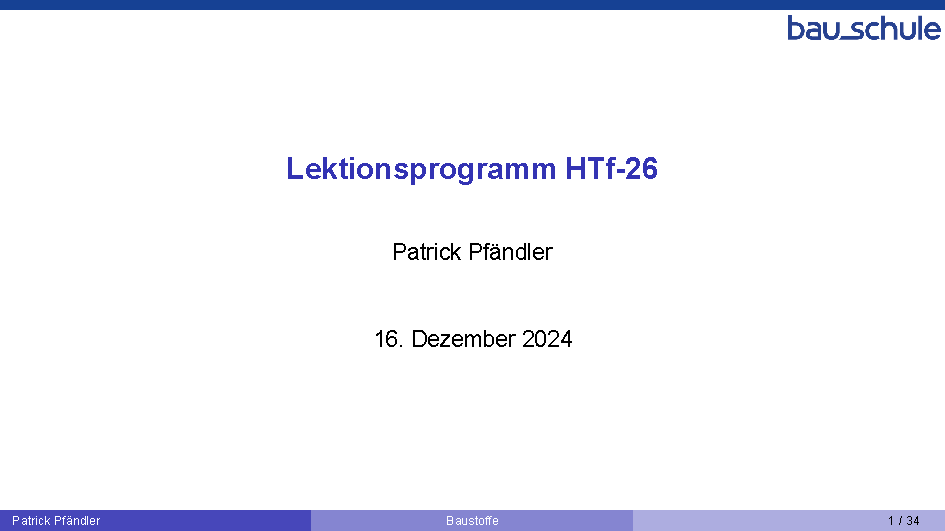
\includepdf[pages=-]{../../HTf-26/KW_51_Programm.pdf}

\end{document}